\section {Vergleich reaktive \& imperative Anwendung}
\label{section:vergleich_reaktiv_imperativ}
Um zu prüfen, ob Leistungsfähigkeit und Skalierbarkeit einer reaktiven, auf dem \newline
\verb|Multi-Reactor-Modell| und \verb|Nonblocking I/O| basierenden,
Anwendung tatsächlich die einer traditionellen, auf dem \verb|Thread-per-Request Modell| und \verb|Blocking I/O| basierenden, Anwendung übertrifft, werden in
diesem Kapitel beide Ansätze hinsichtlich verschiedener Metriken in einem festen Zeitintervall miteinander verglichen.

Dafür werden sowohl die reaktive, als auch die nicht-reaktive Anwendung, in 5 Testreihen, jeweils zwei Lasttests unterzogen:
\begin{enumerate}
    \item Abfrage von statischen Daten
    \item Abfrage von dynamischen Daten (mit Datenbankanbindung)
\end{enumerate}
Dabei wird pro Lasttest eine Reihe an Lasten bzw. \textit{workloads} von einem Client-Host generiert und über eine feste Dauer in kleinen Zeitinvervallen
an einen ausgewählten HTTP-Endpunkt der Anwendung gesendet.
In dieser Zeit wird das Zeitinvervall vom Starten der Anwendung bis zur Beantwortung der ersten Anfrage,
der benötigte Arbeitsspeicher und CPU-Auslastung des Prozesses, der Durchsatz, sowie die Latenz gemessen.

Für Container- und Cloud-Umgebungen eignen sich, primär aus Kostengründen, Anwendungen die, statt auf hohen Durchsatz und lange Laufzeiten, auf
schnelle Startzeiten und geringen Ressourcenverbrauch setzen.
Aus diesem Grund werden die beiden Anwendungen sowohl im \textit{JVM mode} als auch im \textit{native mode}
(siehe Absatz \verb|Quarkus und native image| in Kapitel \ref{subsubsec:frameworks})
den beiden Lasttests unterzogen. Ingesamt ergeben sich also 4 Testszenarien pro Anwendung.

\subsection{Implementierung \& Systemaufbau}
\label{section:implementierung}
Die beiden Anwendungen implementieren mit dem Quarkus-Framework jeweils eine simple REST-Schnittstelle mit HTTP-CRUD Methoden
und einer angebundenen PostgreSQL-Datenbank.
Dabei ist vorallem die HTTP-Schicht von Interesse. Die HTTP-Unterstützung von Quarkus basiert auf einem reaktiven, nicht-blockierenden
Unterbau: der Vert.x Engine (siehe Kapitel \ref{subsubsec:reaktive_systeme}).
Jede HTTP-Anfrage wird auf einem der \textit{event-loop threads} bzw. \textit{IO threads}
verarbeitet und durch eine Routing-Schicht an den Anwendungscode weitergeleitet.
Je nachdem welcher Ansatz zur Implementierung des jeweiligen HTTP-Endpunktes gewählt wurde,
wird der abzuarbeitende Code dann auf einem blockierenden \textit{worker thread}, ganz nach dem \verb|Thread-Per-Request Modell|, aus dem
\textit{worker thread pool} (Servlet, \Gls{jaxrsg}(*)) oder, nach dem \verb|Multi-Reactor-Modell|, weiter auf einem der
\textit{IO threads} (Reactive Routes, Reactive Resteasy) ausgeführt.

\newpage
\begin{figure}[h]
    \centering
    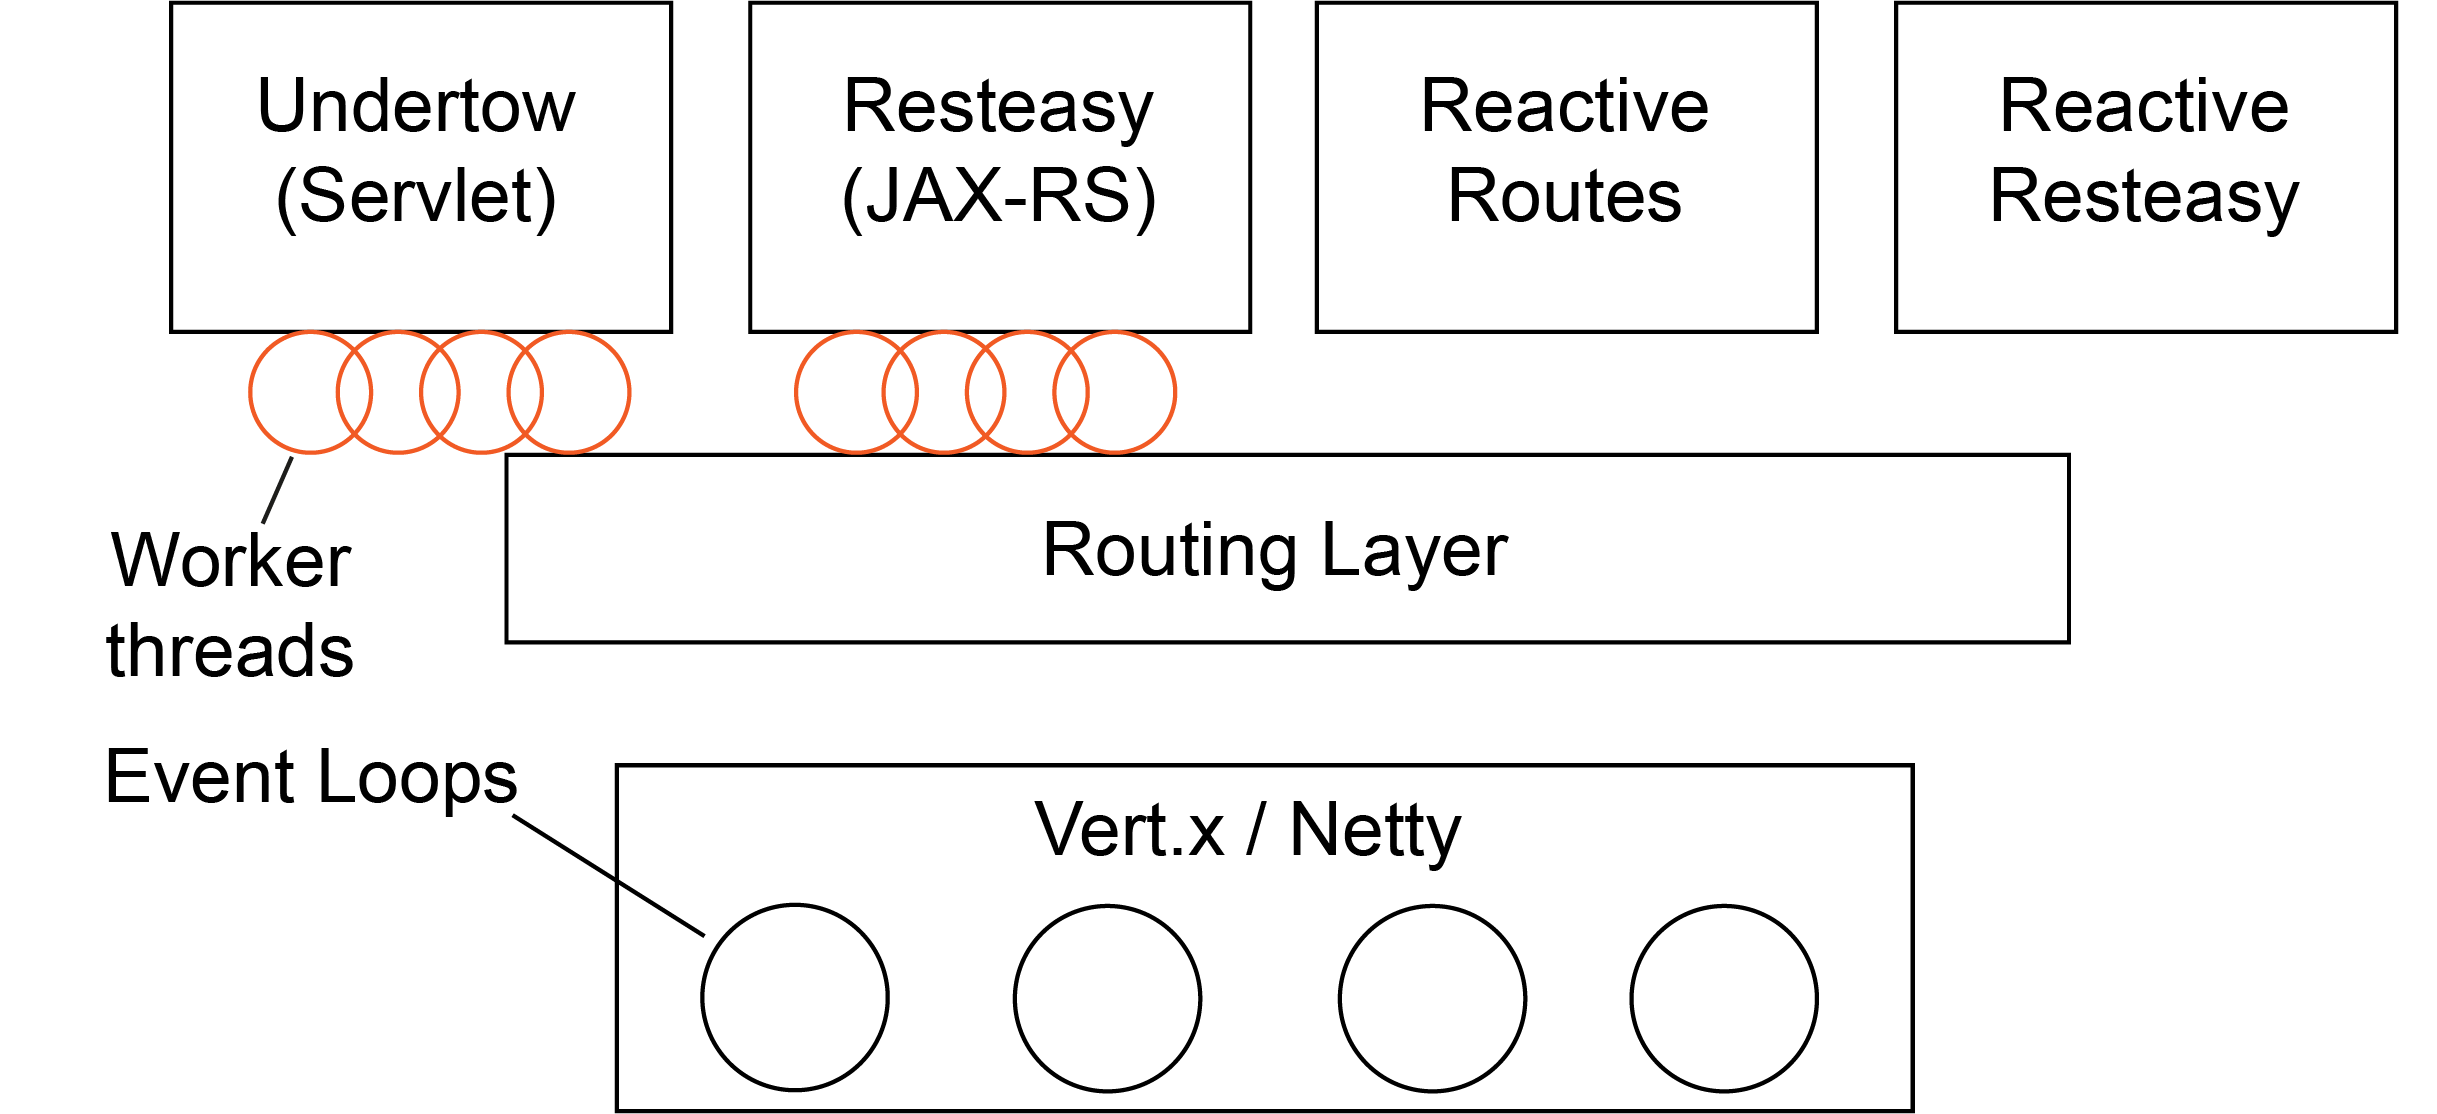
\includegraphics[width=0.9\textwidth]{Quarkus_HTTP_Layer}
    \caption{Quarkus HTTP-Schicht \parencite{QuarkusReactiveRoutes}}
    \label{fig:quarkus_http_schicht}
\end{figure}

Die \textit{IO threads} sind dafür zuständig alle IO-Operationen asynchron auszuführen und die jeweiligen EventListener bzw. Subscriber
auszulösen sobald die Operationen abgeschlossen sind.
Damit sich beide Anwendungen nahe an einer realen Java-EE CRUD REST-API orientieren, haben
sie (zusätzlich zu den grundlegenden Abhängigkeiten des Quarkus-Frameworks) folgende Projekt-Abhängigkeiten:
\begin{itemize}
    \item JAX-RS Implementierung
    \item \Gls{jsong}(*) Unterstützung
    \item PostgreSQL - Datenbanktreiber
    \item \Gls{jpag}(*) Implementierung
\end{itemize}

Diese Abhängigkeiten wurden vom Quarkus Maven-Repository sowohl in blockierender,
als auch in nicht-blockierender, reaktiver und in \verb|native image|-kompatibler Form bereitgestellt: \parencite{MavenQuarkusIO}
% space between the text and the left/right border of its containing cell is set to 18 pt
\setlength{\tabcolsep}{18pt}
% the height of each row is set to 1.5 relative to its default height
\renewcommand{\arraystretch}{1.5}
\begin{table}[ht!]
    \centering
    \begin{tabular}{| c | c | c |}
        \hline
                         & Blockierend      & Nicht-blockierend (reaktiv) \\
        \hline
        JAX-RS           & Resteasy         & Resteasy Reactive           \\
        \hline
        JSON             & Resteasy-Jackson & Resteasy-Reactive-Jackson   \\
        \hline
        Datenbanktreiber & JDBC-Postgresql  & Reactive-Pg-Client          \\
        \hline
        JPA-/ORM         & Hibernate-ORM    & Hibernate-Reactive          \\
        \hline
    \end{tabular}
    \caption{Tabelle mit den Abhängigkeiten beider Applikationen}
    \label{table:dependencies}
\end{table}

In Listing \ref{lst:update_reactive} und \ref{lst:update_blocking} ist jeweils die Update Methode der REST-APIs abgebildet, um den
Unterschied der beiden Paradigmen auf Code-Ebene darzustellen.

Dabei wird versucht eine Entity mit der übergebenen \verb|id| des API-Endpunktes
aus der Datenbank abzurufen und, falls eine Entity mit der \verb|id| gefunden werden konnte, dessen Name mit dem Wert
aus dem Request-Body der Anfrage zu überschreiben. Anschließend wird die Entity mit dem neuen Namen wieder in die Datenbank zurückgeschrieben
und HTTP-Statuscode 422 an den Client zurückgegeben. Falls keine Entity gefunden werden konnte, wird stattdessen
HTTP-Statuscode 404 zurückgegeben.

In der reaktiven Anwendung ist die gesamte Logik, sowie Fehler- und Nullprüfung in einer einzigen Pipeline abgebildet.
Da in diesem Beispiel Mutiny genutzt wird, wird der Rückgabetyp immer als \verb|Uni| oder \verb|Multi|-Objekt eines spezifischen Typs
angegeben. \verb|Uni| repräsentiert dabei einen Datenstrom der entweder ein Element oder ein Fehler-Event emittiert.
\verb|Multi| repräsentiert einen Datenstrom der entweder 0, 1, \verb|n| oder unendlich viele Elemente emittieren kann.
Der \verb|Subscriber| ist in diesem Fall der Aufrufer der \verb|update|-Methode und sorgt dafür, dass die Pipeline überhaupt ausgeführt wird.

Jede \verb|Pipe| bzw. \verb|Processor| der Pipeline der \verb|update|-Methode gibt ein \verb|Uni|, dieses kann entweder
vom Typ \verb|Void| (für null-Werte) oder von der jeweiligen Entität sein, an den Downstream weiter
\footnote{invoke() und call() sind Abkürzungen, um die Lesbarkeit zu verbessern\parencite{MutinyShortcuts}}.

\begin{lstlisting}[caption=Update Methode der reaktiven Anwendung, language=Java, captionpos=b, label=lst:update_reactive]
@PUT
@Path("{id}")
public Uni<Response> update(Long id, Fruit fruit) {
	if (fruit == null || fruit.getName() == null) {
		return Uni.createFrom().item(Response.status(422).build());
	}
	return fruitRepository.findById(id).onItem()
	.ifNotNull().invoke(storedFruit -> storedFruit.setName(fruit.getName())
	).call(storedFruit -> fruitRepository.update(storedFruit))
			.onItem().ifNotNull().transform(storedFruit ->
			Response.ok(storedFruit).build())
			.onItem().ifNull().continueWith(Response.status(Status.NOT_FOUND).build());
}
\end{lstlisting}
\begin{lstlisting}[caption=Update Methode der nicht-reaktiven Anwendung, language=Java, captionpos=b, label=lst:update_blocking]
@PUT
@Path("/{id}")
public Response update(Fruit fruit, @PathParam("id") Long id) {
	if (fruit == null || fruit.getName() == null) {
		return Response.status(422).build();
	}
	Fruit storedFruit = fruitRepository.findById(id);
	if (storedFruit == null) {
		return Response.status(Response.Status.NOT_FOUND).build();
	}
	storedFruit.setName(fruit.getName());
	fruitRepository.update(storedFruit);
	return Response.status(Response.Status.OK).build();
}
\end{lstlisting}

Der Projekt-Code dieser Arbeit kann von GitHub unter \url{https://github.com/ErikSimonsen/quarkus-iothread-workerpool} eingesehen und abgerufen werden.

\subsection{Testumgebung}
\label{section:testumgebung}
Für die Testumgebung werden zwei Systeme benötigt: der Client-Host und der Server-Host.
Dabei muss es sich um UNIX-Systeme handeln, da einige der verwendeten Werkzeuge nur auf diesen Systemen verfügbar sind.
Zudem müssen beide Systeme per SSH von einem (idealerweise vorhandenem) dritten System, dem User-Host
\footnote{Dies kann allerdings auch der Client-Host selber sein}
erreichbar sein, damit dieses den Testablauf in der korrekten Abfolge ausführen kann.
Der Einfachheit halber empfiehlt es sich, dass sich alle Geräte im gleichen Netzwerk befinden.
Beide Anwendungen verwenden Version 1.12.1 des Quarkus Frameworks, welches wiederrum Version 20.1 der GraalVM nutzt.
Um eine reproduzierbare Anwendungsumgebung und Ressourcenallokation zu ermöglichen, laufen beide Anwendungen auf dem Server-Host in
jeweils einem Docker-Container mit fest definierten Ressourcen:
\begin{itemize}
    \item Nutzung von 4 CPU-Kernen
    \item 1024 MB RAM
    \item 256 MB Heap Größe für den Java-Prozess
          \footnote{Seit Java 10 wird automatisch ~1/4 des Speicher Limits des Containers genutzt \parencite{Java10ReleaseNotes}}
\end{itemize}
Der jeweilige Docker-Container für die Postgresql-Datenbank allokiert:
\begin{itemize}
    \item 4 CPU-Kerne
    \item 2048 MB RAM
\end{itemize}

Die Größe des von Vert.x verwendeten \verb|Worker Thread Pools| (siehe Abbildung \ref{fig:quarkus_http_schicht}) beträgt standardmäßig 20 und bleibt
unverändert, die Größe des \verb|Event-Loop Thread Pools| hingegen wird für die Tests manuell auf 8 gesetzt, da die Anwendung durch die Ressourcenallokation
des Docker-Containers nur 4 CPU-Kerne nutzen darf und jeder dieser CPU-Kerne Hyperthreading unterstützt. \footnote{Wodurch jeder physische CPU-Kern über
    zwei logische CPUs verfügt} Damit kann die optimale Verteilung von einem \verb|Event-Loop Thread| bzw. \verb|IO-Thread| pro
logischer CPU erreicht werden.
Standardmäßig wird die Ressourcenbegrenzung durch Container von Vert.x nicht beachtet und die Anzahl der \verb|Event loop|-Threads auf die doppelte
Anzahl der verfügbaren CPU-Kerne des Container-Hosts gesetzt, weswegen es für ressourcenbegrenzte Container der beschriebenen Korrektur bedarf.
Der \verb|Worker Thread Pool| wird vom \verb|Thread-per-Request Modell| bzw. \verb|Blocking I/O| genutzt, während der \verb|Event-Loop Thread Pool| von der
reaktiven Anwendung bzw. \verb|Nonblocking I/O| genutzt wird.

Die Anwendung, die auf dem Client-Host die \textit{work load} für die beiden zu testenden Anwendungen generiert,
nutzt in dieser Testumgebung 4 Threads.
\footnote{Welche Laufzeitumgebungen und Tools für die Tests auf den jeweiligen Hosts vorhanden sein müssen, und wie diese installiert werden
    wird in der README.md-Datei des Projektverzeichnisses beschrieben.}

Da die Messergebnisse je nach verwendeter Hardware der Client- und Server-Hosts durchaus variieren können werden im Folgenden
die Systemspezifikationen der verwendeten Systeme des Authors gelistet:
\begin{table}[ht!]
    \centering
    \begin{tabular}{| c | c |}
        \hline
        Server-Host                                                  \\
        \hline
        CPU's          & AMD Ryzen 7 2700x eight-core processor x 16 \\
        \hline
        RAM            & 16GB                                        \\
        \hline
        Speicher       & 1,5 TB                                      \\
        \hline
        Betriebssystem & Fedora 34 (Workstation Edition)             \\
        \hline
        Kernel         & Linux version \verb|5.12.14-300.fc34.x86_64|   \\
        \hline
    \end{tabular}
    \caption{Systemspezifikationen der verwendeten Server-Maschine}
    \label{table:system_host}
\end{table}

\begin{table}[ht!]
    \centering
    \begin{tabular}{| c | c |}
        \hline
        Client-Host                                                \\
        Hardware       & Acer Aspire VN7-591G                      \\
        \hline
        CPU            & Intel® Core™ i5-4210H CPU @ 2.90GHz × 4   \\
        \hline
        RAM            & 8GB                                       \\
        \hline
        Speicher       & 500 GB                                    \\
        \hline
        Betriebssystem & Fedora 34 (Workstation Edition)           \\
        \hline
        Kernel         & Linux version \verb|5.12.14-300.fc34.x86_64| \\
        \hline
    \end{tabular}
    \caption{Systemspezifikationen der verwendeten Client-Maschine}
    \label{table:system_client}
\end{table}

\subsection{Testvorgehen / Testaufbau}
\label{section:vorgehen}
Der im Folgenden erläuterte Versuchsaufbau basiert auf einer, vom Autor erweiterten, Architektur die vom Quarkus-Entwicklerteam
zur Erstellung von verschiedenen Benchmarks für den Quarkus Technologie-Stack genutzt wurde.
\parencite{QuarkusBlog, QuarkusJohnaohara}

Um den gesamten Versuchsablauf zu automatisieren und über mehrere Server zu steuern wird ein Tool namens qDup eingesetzt.
Damit können Shell-Kommandos als Skripte gruppiert, und verschiedenen Hosts je nach Rolle zugewiesen werden.
\footnote{Die qDup Skripte mit dem gesamten Testablauf können im Verzeichnis \textit{/scripts/qDup} des Quellcodeverzeichnisses eingesehen und
    angepasst werden.}
Um dem Ablauf korrekt zu steuern werden Signale definiert die ein Host sendet, und auf die die anderen Hosts warten um ihrerseits
weitere Skripte auszuführen.
\footnote{Beispielsweise sollte der Server-Host erst anfangen den Java-Prozess zu überwachen, sobald der Client-Host die \textit{workload}
    generiert und nicht bereits davor}

Wie bereits in \ref{section:testumgebung} angedeutet, nutzt qDup SSH um auf die jeweilige Hosts zuzugreifen.

Im ersten Schritt \textit{build applications} wird auf dem Server-Host das Quellcodeverzeichnis geklont und beide Anwendungen werden, für
ein einfaches Deployment in den Docker-Container, jeweils als \gls{uber-jar}(*) und \verb|native image| gebaut.

Anschließend wird über ein JavaScript-Skript, welches in der Laufzeitumgebung Node.js läuft,
die \verb|Mean Start Time to First Request|, also das durchschnittliche Zeitintervall zwischem dem Start einer Anwendung bis
zur Verarbeitung der ersten Anfrage, mehrfach gemessen und als Textdatei gespeichert.
Dabei wird die gebaute Anwendung, ohne Docker-Container, auf dem Server-Host gestartet und die Zeit genommen. Anschließend werden in einer Schleife
solange Anfragen an einen Endpunkt der Anwendung gestellt bis das Ergebnis ein Statuscode 200 ist, was den Endpunkt der Messung markiert.
Aus den gemessenen Startzeiten wird in der Auswertung der Daten anschließend der Durchschnitt gebildet, um somit die \verb|Mean Start Time to First Request|
der Anwendung zu erhalten.

Darüber hinaus werden die Docker-Container der Datenbank
\footnote{Nur beim Test mit dynamischen Daten} und der beiden REST-APIs gebaut.

Beim zweiten Schritt \textit{run applications} wird der Docker-Container der jeweiligen Anwendung gestartet und anschließend signalisiert,
dass die Anwendung nun bereit ist.
Daraufhin wird auf dem Client-Host das Skript \textit{generate load} gestartet.
Die \textit{workload} ist hier definiert als die Anzahl der, an den Server-Host, versendeten \textit{HTTP-Anfragen pro Sekunde}.
Für das Generieren und Übermitteln der \textit{workload} wird das Werkzeug \textit{wrk2} genutzt, welches das
bewährte HTTP-Benchmarking Tool \textit{wrk} um folgende Funktionen erweitert:
\begin{enumerate}
    \item Konstanter \textit{workload} Durchsatz
    \item Korrekteres Messverfahren der Antwort-Latenz durch Vermeidung von \verb|Coordinated Omission|
    \item Hochexaktes Messen durch \Glsuseri{hdrHistogramm}(*)
\end{enumerate}\parencite{Wrk2, Wrk}

\paragraph{Coordinated Omission Problem}
Der Begriff \verb|Coordinated Omission Problem| wurde von Gil Tene, CTO und Mitgründer von Azul Systems, um 2012 geprägt.
Koordinierte Auslassung beschreibt in diesem Kontext das Problem, wenn ein Messsystem sich mit dem zu messenden System versehentlich so koordiniert,
dass es vermieden wird Ausreißer zu messen.

Viele Lastgeneratoren (load generator) berechnen die Latenz für eine Anfrage als die vergangene Zeit zwischen dem Senden des ersten Bytes einer Anfrage
bis zum Erhalt der kompletten Antwort. Während dieses Modell die tatsächliche Bearbeitungszeit individueller Anfragen korrekt misst,
liegt dabei ein starker koordinierter Auslassungseffekt vor,
wodurch die meisten Artefakte mit hoher Latenz, die der gemessene Server aufweist, ignoriert werden.
Da jede Verbindung erst anfängt eine neue Anfrage zu senden, nachdem eine Antwort bezüglich der vorherigen Anfrage erhalten wurde,
resultieren Antworten mit hoher Latenz darin, dass der Lastgenerator in einem bestimmten Zeitintervall weniger Anfragen an den Server schickt als in einer
Phase niedriger Latenz, da die weiteren Anfragen alle verzögert werden. Ähnlich wie bei \verb|Event Loops| \textit{blockieren}
Anfragen mit hoher Latenz also das Absenden weiterer Anfragen.
Dadurch koordiniert der Lastgenerator sich unbeabsichtigt mit dem Server um weitere Messungen während Phasen hoher Latenz zu vermeiden, da die Last die der Server
in dieser Phase abzuarbeiten hat deutlich geringer ist als bei niedriger Latenz. Das Hauptproblem ist also, dass die Last die der Server empfängt
nicht durchgehend \verb|konstant| ist, sondern von der Antwortszeit des Servers abhängt \parencite{mci/Friedrich2017}.
\newline\newline
\verb|Wrk2|, dessen Author auch Gil Tene ist, umgeht das \verb|Coordinated Omission Problem| in dem es eine konstante Durchsatzlast (als Befehlsargument) mit
einer Latenzmessung, die den beabsichtigten konstanten Durchsatz berücksichtigt, kombiniert. Anstatt dabei die Antwortlatenz ab dem Zeitpunkt zu messen,
zu dem die tatsächliche Übertragung einer Anfrage aufgetreten ist, misst wrk2 die Antwortlatenz ab dem Zeitpunkt, zu dem die Übertragung,
gemäß dem für den Durchlauf konfigurierten konstanten Durchsatz, hätte erfolgen \textit{sollen} bis zum Erhalt der vollständigen Antwort\parencite{Wrk2}.

Pro Test (siehe Anfang des Kapitels \ref{section:vergleich_reaktiv_imperativ}) werden Benchmarks für eine ganze Reihe an \textit{workloads} gemessen.
Jede \textit{workload} wird sekündlich über einen Zeitraum von 60 Sekunden über 100 offene HTTP-Verbindungen an den Server-Host übermittelt.
In den Tests nutzt \verb|wrk2| für das Generieren und Übermitteln der \textit{workload}, sowie das Messen der Antwortszeit
4 Threads.
\newline\newline
Damit der Anwendungscode des angesteuerten HTTP-Endpunkts durch den JIT-Compiler der JVM (siehe Absatz \verb|Quarkus und native image| in Kapitel
\ref{subsubsec:frameworks}) optimiert wird, findet pro \textit{workload} vor der eigentlichen Mess-Phase eine identische Warmup-Phase statt.

Listing \ref*{lst:generateLoad} zeigt den Aufruf von \verb|wrk2| mit den beschriebenen Parametern in der Warmup- und Mess-Phase,
\verb|${RUN_RATE}| enthält dabei die \textit{workload}.
\footnote{Das manuelle Kompilieren des Quellcodes von wrk2 produziert, wie wrk auch, ein executable namens wrk}

\begin{lstlisting}[caption=Auszug des qDup Skripts generate load, captionpos=b, label=lst:generateLoad]
- signal: ${{RUNTIME.name}}-${{RUN_RATE}}-WARM-UP-START
- sh: wrk -t 4 -c 100 -d 60s -R ${{RUN_RATE}} ${{TEST_DYNAMIC_ENDPOINT}} > ${{CLIENT_FILE_PATH}}/output/${{RUNTIME.name}}-${{RUN_RATE}}-WARM-UP.wrk2.out
- signal: ${{RUNTIME.name}}-${{RUN_RATE}}-WARM-UP-END
- sh: sleep 5s
- signal: ${{RUNTIME.name}}-${{RUN_RATE}}-MEASURE-START
- sh: wrk -t 4 -c 100 -d 60s -R ${{RUN_RATE}} --latency ${{TEST_DYNAMIC_ENDPOINT}} > ${{CLIENT_FILE_PATH}}/output/${{RUNTIME.name}}-${{RUN_RATE}}-MEASURE.wrk2.out
- signal: ${{RUNTIME.name}}-${{RUN_RATE}}-MEASURE-END
   \end{lstlisting}

Die Ausgabe von wrk2 enthält Informationen zur \Gls{latenz}\footnote{Pro verwendetem Thread und Gesamt},
zum \Gls{durchsatz} und der \Gls{perzentile}(*) der \Gls{latenz}, welches durch ein \Gls{hdrHistogramm} dargestellt wird.
Listing \ref*{lst:wrk-listing} zeigt die umgeleitete Ausgabe von \textit{wrk} ohne die genaue Darstellung der Perzentile.

\begin{lstlisting}[caption=Beispiel für Ausgabe von wrk,captionpos=b, label=lst:wrk-listing]
Running 1m test @ http://erik-pc.local:8080/greeting/Bob
4 threads and 100 connections
Thread calibration: mean lat.: 310.434ms, rate sampling interval: 1047ms
Thread calibration: mean lat.: 330.365ms, rate sampling interval: 1127ms
Thread calibration: mean lat.: 298.671ms, rate sampling interval: 994ms
Thread calibration: mean lat.: 333.465ms, rate sampling interval: 1123ms
Thread Stats   Avg      Stdev     Max   +/- Stdev
	Latency     1.76s   738.93ms   4.12s    62.98%
	Req/Sec    28.58k   633.82    30.09k    66.49%
6839722 requests in 1.00m, 476.17MB read
Requests/sec: 113929.77
Transfer/sec:      7.93MB
\end{lstlisting}

Bevor die Warmup-Phase und die Belastungs-Phase vom Client-Host ausgeführt werden, wird dem Server-Host signalisiert, dass
er das Skript \textit{capture platform stats} ausführen soll.
In diesem Skript wird die Observation des Anwendungs-Prozesses durch das Kommandozeilenprogramm \verb|top| gestartet.
\verb|Top| wird dabei im Batch-Modus gestartet mit einer Wiederholrate von einer Sekunde.

Die Prozess-Zeile der Ausgabe von \verb|top| enthält eine Vielzahl an Informationen zu dem beobachteten Prozess, von besonderem
Interesse sind hierbei die CPU-Auslastung und der verwendete Arbeitsspeicher des Prozesses. \parencite{linuxTopManual}

\begin{lstlisting}[language=sh, caption=Auszug des qDup Skripts capture-platform-stats, captionpos=b]
- wait-for: ${{RUNTIME.name}}-${{RUN_RATE}}-WARM-UP-START
- sh: top -b  -d 1 -p ${{RUN.JAVA_APP_PID}} | grep java > ${{SERVER_FILE_PATH}}/output/${{RUNTIME.name}}-${{RUN_RATE}}-WARM-UP-top.out &
- sh: export TOP_PID=$!
- wait-for: ${{RUNTIME.name}}-${{RUN_RATE}}-WARM-UP-END
- sh: kill -9 $TOP_PID
- wait-for: ${{RUNTIME.name}}-${{RUN_RATE}}-MEASURE-START
- sh: top -b  -d 1 -p ${{RUN.JAVA_APP_PID}} | grep java > ${{SERVER_FILE_PATH}}/output/${{RUNTIME.name}}-${{RUN_RATE}}-MEASURE-top.out &
- sh: export TOP_PID=$!
- wait-for: ${{RUNTIME.name}}-${{RUN_RATE}}-MEASURE-END
- sh: kill -9 $TOP_PID
  \end{lstlisting}

Im letzten Schritt werden alle Ausgaben über SSH vom Client- und Server-Host auf den User-Host der das qDup Skript ausgeführt hat kopiert.

\begin{figure}[ht]
    \centering
    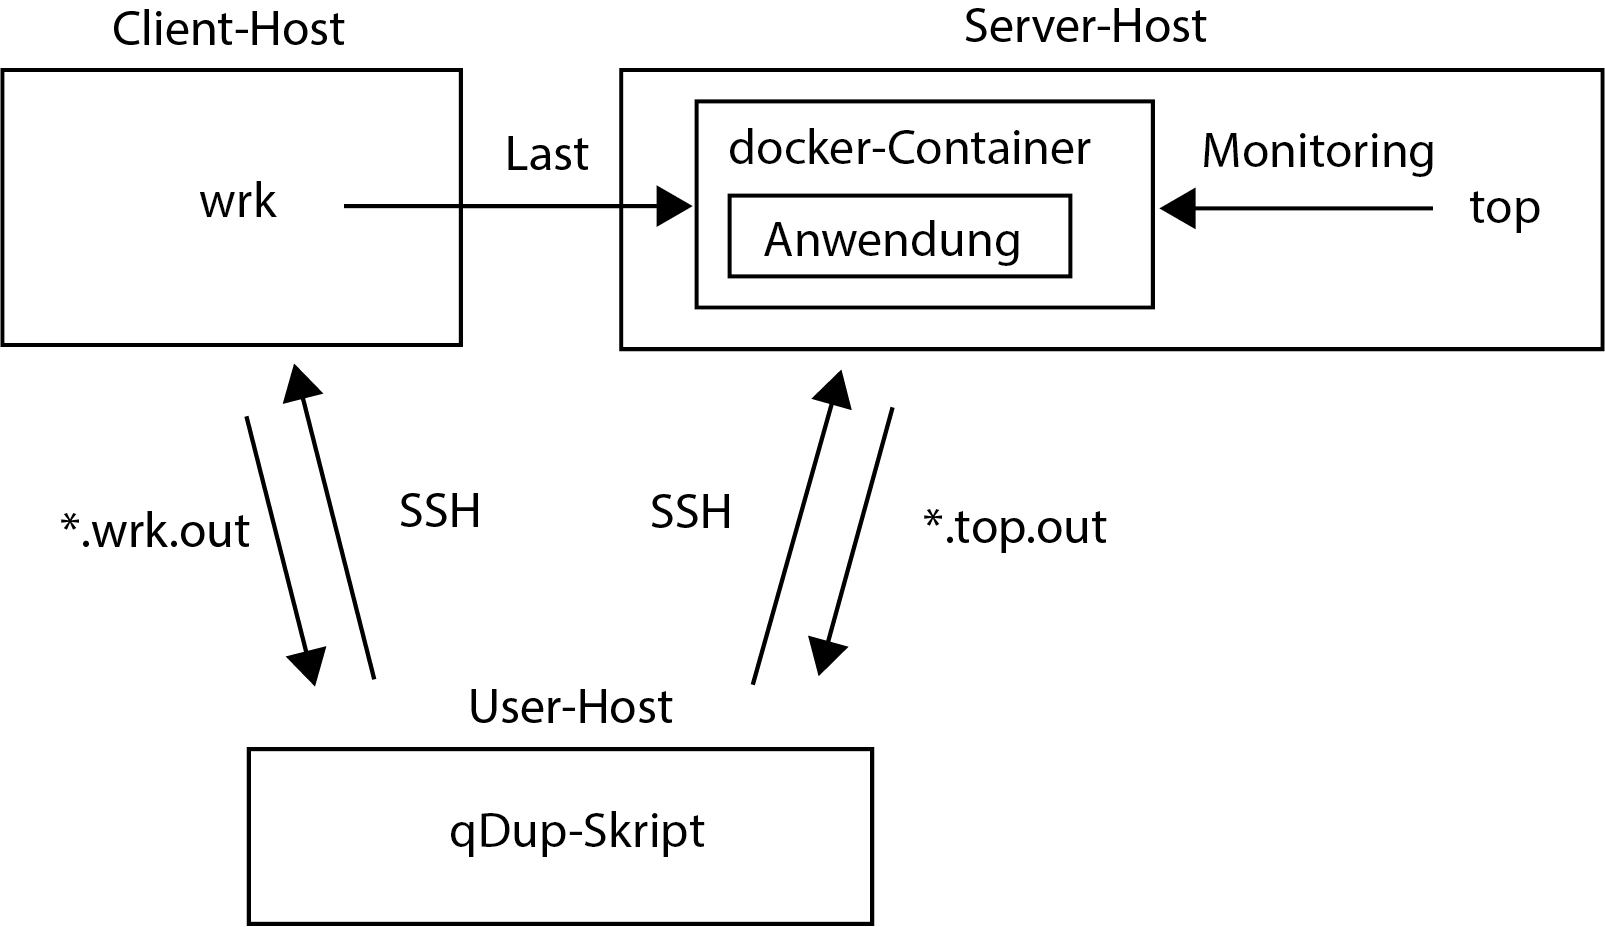
\includegraphics[width=0.7\textwidth]{Testaufbau}
    \caption{Testaufbau}
\end{figure}

In einem Bash-Skript werden anschließend die Ausgaben von \verb|top| und \verb|wrk| für jede einzelne \verb|workload| eines Tests
über ein Java-Skript, das mit dem Tool \textit{JBang} ausgeführt wird \footnote{JBang erlaubt das direkte Ausführen von .java Dateien},
eingelesen, analysiert und jeweils der Durchschnitt, das Minimum und das Maximum des Durchsatzes, Speicherverbrauches und CPU-Auslastung pro Last ermittelt.
Diese werden dann für die visuelle Darstellung in eine \verb|.json|-Datei geschrieben.
Zu guter Letzt werden die aufbereiteten Daten durch die Node.js-Bibliothek \textit{d3node-linechart} als Liniendiagramme visuell dargestellt.

\subsection{Test: Statische Daten}
\label{subsection:statische_daten}
Im Folgenden werden die Testresultate der \verb|2.| Testreihe dargestellt, erläutert und anschließend zusammengefasst.
Die Ergebnisse der anderen Testreihen liegen in den gleichen Größenordnungen und können im Projektverzeichnis unter \verb|results/data| und \verb|results/graphs| eingesehen werden.
Der Lasttest mit statischen Daten wird ohne Datenbankanbindung durchgeführt und der angesteuerte Endpunkt \verb|/greeting/{name}| gibt bei beiden Anwendungen
jeweils einen statischen String zurück. Wie bereits zu Beginn des Kapitels erwähnt, wird jede Anwendung sowohl im \verb|JVM mode|, als auch im
\verb|native mode| getestet.
Die qDup-Skripte befinden sich im Projektverzeichnis im Verzeichnis \verb|scripts/benchmark-jvm-static.yaml| und
\verb|scripts/benchmark-native-static.yaml|.

\subsubsection{JVM mode}
\label{subsubsec:static_jvm_mode}
Wie aus Listing \ref{lst:starttimes_jvm_static} berechnet werden kann, liegt die durchschnittliche Zeit vom Start der Anwendung bis zur
Bearbeitung der ersten Anfrage ohne Datenbankanbindung bei einer reaktiven Anwendung im \verb|JVM mode| bei 1353 ms und bei einer
blockierenden Anwendung bei 1516,6 ms.
\begin{lstlisting}[caption=5 gemessene Startzeiten bis zur Bearbeitung der ersten Anfrage als JVM-Anwendungen: links ist die reaktive 
    Anwendung und rechts die blockierende Anwendung, captionpos=b, label=lst:starttimes_jvm_static]
    1356 ms     1531 ms
    1337 ms     1504 ms
    1315 ms     1495 ms
    1349 ms     1509 ms
    1408 ms     1544 ms
\end{lstlisting}

In Abbildung \ref{fig:jvm_static_mean_response} wird die durchschnittlich gemessene Latenz für jede getestete \verb|workload|,
in diesem Diagramm als Durchsatz beschrieben, dargestellt.
Die höchste getestete \verb|workload| beträgt bei der reaktiven Anwendung \textbf{142.000} Anfragen/Sekunde und bei der
nicht-reaktiven Anwendung \textbf{71.000} Anfragen/Sekunde.

Der maximale serverseitige Durchsatz der nicht-reaktiven Anwendung beträgt ~\textbf{69.000} Anfragen/Sekunde mit einer
Latenz von ~217,5 ms und
die reaktive Anwendung erreicht ~\textbf{140.000} Anfragen/Sekunde bei einer durchschnittlichen Latenz von ~646,5 ms.
Bei höheren Lasten steigt die durchschnittliche Latenz auf deutlich über eine Sekunde, weswegen der Durchsatz stagniert.

Die reaktive Anwendung erreicht also in der vorliegenden Testumgebung für einen trivialen
Endpunkt mit statischen Daten mehr als den doppelten Durchsatz.
\newpage
\begin{figure}[ht!]
    \includegraphics[width=1.0\textwidth]{run2/jvm-static/mean-response-vs-throughput}
    \caption{Test mit statischen Ressourcen im JVM mode: Durchschnittliche Latenz jeder Last}
    \label{fig:jvm_static_mean_response}
\end{figure}
Abbildung \ref{fig:jvm_static_mean_rss} stellt den durchschnittlich allokierten Speicher des jeweiligen Anwendungsprozesses
im Hauptspeicher für jede \verb|workload| dar. Der allokierte Speicher für die genannten maximalen Durchsätze beträgt dabei bei
der reaktiven Anwendung ~\verb|580 MB| und bei der blockierenden, nicht-reaktiven Anwendung ~\verb|843 MB|.
\newpage
\begin{figure}[ht!]
    \includegraphics[width=1.0\textwidth]{run2/jvm-static/mean-rss-vs-throughput}
    \caption{Test mit statischen Ressourcen im JVM mode: Allokierter Hauptspeicher pro workload}
    \label{fig:jvm_static_mean_rss}
\end{figure}
Zu guter Letzt wird in Abbildung \ref{fig:jvm_static_avg_cpu} die durchschnittlich gemessene CPU-Auslastung für jede \verb|workload|
dargestellt. Bei der nicht-reaktiven Anwendung wird eine durschnittliche CPU-Auslastung von 98\% bereits bei einer Last von
50.000 Anfragen/Sekunde erreicht, die reaktive Anwendung hingegen erreicht diese Auslastung erst bei 110.000 Anfragen/Sekunde.
\newpage
\begin{figure}[ht!]
    \centering
    \includegraphics[width=1.0\textwidth]{run2/jvm-static/average-cpu-vs-throughput}
    \caption{Test mit statischen Ressourcen im JVM mode: CPU Auslastung pro workload}
    \label{fig:jvm_static_avg_cpu}
\end{figure}

In Tabelle \ref{table:static_jvm_measurement_results} werden die Resultate der gemessenen Benchmarks zusammengefasst
und zueinander ins Verhältnis gesetzt. Im JVM mode mit statischen Ressourcen erreicht die reaktive Anwendung
eine 11,8\% schnellere durchschnittliche Startzeit bis vollständigen Bearbeitung der ersten Anfrage, sowie
einen um 31,2\% geringeren Speicherverbrauch.
Darüber hinaus wird ein um etwa 102\% höherer maximaler Durchsatz erzielt, bevor die Latenz eine Sekunde übersteigt, und
es können 120\% mehr Anfragen pro Sekunde verarbeitet werden bis die CPU Auslastung, mit dem in Tabelle \ref{table:system_host}
genannten CPU, bei 4 Kernen 98\% erreicht.

\begin{table}[ht!]
    \begin{tabular}{|l | c | c | c|}
        \hline
        Run 2 - JVM mode - static & Blockierend & Reaktiv & Verhältnis \\
        \hline
        \makecell[l]{Durchschn. Startzeit bis                          \\erste Anfrage (ms)} & 1516,6      & 1353  & 89,2\%     \\
        \hline
        Max. allokierter RAM (MB) & 843         & 580     & 68,8\%     \\
        \hline
        Max. Durchsatz (req/sec)  & 69.000      & 140.000 & 202\%      \\
        \hline
        \makecell[l]{CPU Auslastung bei 98\%                           \\ (req/sec)} & 50.000 & 110.000 & 220\%  \\
        \hline
    \end{tabular}
    \caption{Verhältnis der gemessenen Benchmarks für beide Anwendungen im JVM mode mit statischen Ressourcen}
    \label{table:static_jvm_measurement_results}
\end{table}

\subsubsection{native mode}
\label{subsubsec:static_native_mode}
Wie aus Listing \ref{lst:starttimes_native_static} berechnet werden kann, liegt die durchschnittliche Zeit vom Start der Anwendung bis
zur Bearbeitung der ersten Anfrage ohne Datenbankanbindung sowohl bei einer reaktiven Anwendung, als auch bei einer blockierenden
Anwendung im \verb|native mode| bei 27,6 ms.
\begin{lstlisting}[caption=5 gemessene Startzeiten bis zur Bearbeitung der ersten Anfrage als native executables: links ist die
     reaktive Anwendung und rechts die blockierende Anwendung, captionpos=b, label=lst:starttimes_native_static]
    27 ms     27 ms
    27 ms     27 ms
    28 ms     29 ms
    29 ms     27 ms
    27 ms     28 ms
\end{lstlisting}
In Abbildung \ref{fig:native_static_mean_response} wird die durchschnittlich gemessene Latenz für jede getestete \verb|workload|,
in diesem Diagramm als Durchsatz beschrieben, dargestellt.
Die höchste getestete \verb|workload| beträgt bei der reaktiven Anwendung \textbf{76.000} Anfragen/Sekunde und bei der
nicht-reaktiven Anwendung \textbf{39.000} Anfragen/Sekunde.

Der maximale serverseitige Durchsatz der nicht-reaktiven Anwendung beträgt ~\textbf{37.000} Anfragen/Sekunde mit einer
Latenz von ~283,3 ms und
die reaktive Anwendung erreicht ~\textbf{74.000} Anfragen/Sekunde bei einer durchschnittlichen Latenz von ~680,6 ms.
Bei höheren Lasten steigt die Latenz auf deutlich über eine Sekunde, weswegen der Durchsatz stagniert.

Die reaktive Anwendung erreicht also in der vorliegenden Testumgebung für einen trivialen
Endpunkt mit statischen Daten im \verb|native mode| den doppelten Durchsatz.
\newpage
\begin{figure}[ht!]
    \centering
    \includegraphics[width=1.0\textwidth]{run2/native-static/mean-response-vs-throughput}
    \caption{Test mit statischen Ressourcen im native mode: Durchschnittliche Latenz jeder Last}
    \label{fig:native_static_mean_response}
\end{figure}
Abbildung \ref{fig:native_static_mean_rss} stellt den durchschnittlich allokierten Speicher des jeweiligen Anwendungsprozesses
im Hauptspeicher für jede \verb|workload| dar. Der allokierte Speicher für die genannten maximalen Durchsätze beträgt dabei bei
der reaktiven Anwendung ~\verb|364 MB| und bei der blockierenden, nicht-reaktiven Anwendung ~\verb|564 MB|.
\newpage
\begin{figure}[ht!]
    \centering
    \includegraphics[width=1.0\textwidth]{run2/native-static/mean-rss-vs-throughput}
    \caption{Test mit statischen Ressourcen im native mode: Allokierter Hauptspeicher pro workload}
    \label{fig:native_static_mean_rss}
\end{figure}

Zu guter Letzt wird in Abbildung \ref{fig:native_static_avg_cpu} die durchschnittlich gemessene CPU-Auslastung für jede \verb|workload|
dargestellt. Bei der nicht-reaktiven Anwendung wird eine durschnittliche CPU-Auslastung von 98\% bereits bei einer Last von
34.000 Anfragen/Sekunde erreicht, die reaktive Anwendung hingegen erreicht diese Auslastung erst bei 50.000 Anfragen/Sekunde.
\newpage
\begin{figure}[ht!]
    \centering
    \includegraphics[width=1.0\textwidth]{run2/native-static/average-cpu-vs-throughput}
    \caption{Test mit statischen Ressourcen im native mode: CPU Auslastung pro workload}
    \label{fig:native_static_avg_cpu}
\end{figure}

In Tabelle \ref{table:static_native_measurement_results} werden die Resultate der gemessenen Benchmarks zusammengefasst
und zueinander ins Verhältnis gesetzt. Im JVM mode mit statischen Ressourcen erreicht die reaktive Anwendung
die gleiche durchschnittliche Startzeit bis vollständigen Bearbeitung der ersten Anfrage, sowie
einen um 35,5\% geringeren Speicherverbrauch.
Darüber hinaus wird ein um etwa 100\% höherer maximaler Durchsatz erzielt, bevor die Latenz eine Sekunde übersteigt, und
es können 47\% mehr Anfragen pro Sekunde verarbeitet werden bis die CPU Auslastung, mit dem in Tabelle \ref{table:system_host}
genannten CPU, bei 4 Kernen 98\% erreicht.

\begin{table}[ht!]
    \begin{tabular}{|l | c | c | c|}
        \hline
        Run 2 - native mode - static & Blockierend & Reaktiv & Verhältnis \\
        \hline
        \makecell[l]{Durchschn. Startzeit bis                             \\erste Anfrage (ms)} &   27,6    &  27,6  &   100\%   \\
        \hline
        Max. allokierter RAM (MB)    & 564         & 364     & 64,5\%     \\
        \hline
        Max. Durchsatz (req/sec)     & 37.000      & 74.000  & 200\%      \\
        \hline
        \makecell[l]{CPU Auslastung bei 98\%                              \\ (req/sec)} & 34.000 & 50.000 & 147\%  \\
        \hline
    \end{tabular}
    \caption{Verhältnis der gemessenen Benchmarks für beide Anwendungen im native mode mit statischen Ressourcen}
    \label{table:static_native_measurement_results}
\end{table}
\newpage
\subsection{Test: Datenbankzugriffe}
\label{section:datenbankzugriffe}
Im Folgenden werden die Testresultate der \verb|4.| Testreihe dargestellt und erläutert.
Die Ergebnisse der anderen Testreihen können im Projektverzeichnis unter \verb|results/data| und \verb|results/graphs| eingesehen werden.
Der Lasttest mit dynamischen Daten wird mit Datenbankanbindung durchgeführt und der angesteuerte Endpunkt \verb|/fruits| gibt bei beiden Anwendungen
jeweils alle Elemente der Tabelle \textit{fruits} zurück. Wie bereits zu Beginn des Kapitels erwähnt, wird jede Anwendung sowohl im \verb|JVM mode|, als auch im
\verb|native mode| getestet, die qDup-Skripte befinden sich im Projektverzeichnis im Verzeichnis \verb|scripts/benchmark-jvm-db.yaml| und
\verb|scripts/benchmark-native-db.yaml|.

\subsubsection{JVM mode}
\label{subsubsec:dynamic_jvm_mode}
Wie aus Listing \ref{lst:starttimes_jvm_dynamic} berechnet werden kann, liegt die durchschnittliche Zeit vom Start der Anwendung bis zur
Bearbeitung der ersten Anfrage mit Datenbankanbindung bei einer reaktiven Anwendung im \verb|JVM mode| bei 1327 ms und bei einer
blockierenden Anwendung bei 1658,8 ms.

\begin{lstlisting}[caption=5 gemessene Startzeiten bis zur Bearbeitung der ersten Anfrage als JVM-Anwendungen: links ist die reaktive
     Anwendung und rechts die blockierende Anwendung, captionpos=b, label=lst:starttimes_jvm_dynamic]
    1305 ms     1664 ms
    1364 ms     1684 ms
    1357 ms     1616 ms
    1307 ms     1638 ms
    1302 ms     1692 ms
\end{lstlisting}

In Abbildung \ref{fig:jvm_dynamic_mean_response} wird die durchschnittlich gemessene Latenz für jede getestete \verb|workload|,
in diesem Diagramm als Durchsatz beschrieben, dargestellt.
Die höchste getestete \verb|workload| beträgt bei der reaktiven Anwendung \textbf{37.000} Anfragen/Sekunde und bei der
nicht-reaktiven Anwendung \textbf{28.000} Anfragen/Sekunde.

Der maximale serverseitige Durchsatz der nicht-reaktiven Anwendung beträgt ~\textbf{27.000} Anfragen/Sekunde mit einer
Latenz von ~913,6 ms und
die reaktive Anwendung erreicht ~\textbf{36.000} Anfragen/Sekunde bei einer durchschnittlichen Latenz von ~484,8 ms.
Bei höheren Lasten steigt die Latenz auf deutlich über eine Sekunde, weswegen der Durchsatz stagniert.
\newpage
\begin{figure}[ht!]
    \centering
    \includegraphics[width=1.0\textwidth]{run4/jvm-db/mean-response-vs-throughput}
    \caption{Test mit dynamischen Ressourcen im JVM mode: Durchschnittliche Latenz jeder Last}
    \label{fig:jvm_dynamic_mean_response}
\end{figure}
Abbildung \ref{fig:jvm_dynamic_mean_rss} stellt den durchschnittlich allokierten Speicher des jeweiligen Anwendungsprozesses
im Hauptspeicher für jede \verb|workload| dar. Der allokierte Speicher für die genannten maximalen Durchsätze beträgt dabei bei
der reaktiven Anwendung ~\verb|685 MB| und bei der blockierenden, nicht-reaktiven Anwendung ~\verb|709 MB|.
\newpage
\begin{figure}[ht!]
    \centering
    \includegraphics[width=1.0\textwidth]{run4/jvm-db/mean-rss-vs-throughput}
    \caption{Test mit dynamischen Ressourcen im JVM mode: Allokierter Hauptspeicher pro workload}
    \label{fig:jvm_dynamic_mean_rss}
\end{figure}

Zu guter Letzt wird in Abbildung \ref{fig:jvm_dynamic_avg_cpu} die durchschnittlich gemessene CPU-Auslastung für jede \verb|workload|
dargestellt. Bei der nicht-reaktiven Anwendung wird eine durschnittliche CPU-Auslastung von 98\% bereits bei einer Last von
20.000 Anfragen/Sekunde erreicht, die reaktive Anwendung hingegen erreicht diese Auslastung erst bei 36.000 Anfragen/Sekunde.
\newpage
\begin{figure}[ht!]
    \centering
    \includegraphics[width=1.0\textwidth]{run4/jvm-db/average-cpu-vs-throughput}
    \caption{Test mit dynamischen Ressourcen im JVM mode: CPU Auslastung pro workload}
    \label{fig:jvm_dynamic_avg_cpu}
\end{figure}

In Tabelle \ref{table:dynamic_jvm_measurement_results} werden die Resultate der gemessenen Benchmarks zusammengefasst
und zueinander ins Verhältnis gesetzt. Im JVM mode mit statischen Ressourcen erreicht die reaktive Anwendung
eine 20,1\% schnellere durchschnittliche Startzeit bis vollständigen Bearbeitung der ersten Anfrage, sowie
einen um 3,4\% geringeren Speicherverbrauch.
Darüber hinaus wird ein um etwa 33\% höherer maximaler Durchsatz erzielt, bevor die Latenz eine Sekunde übersteigt, und
es können 80\% mehr Anfragen pro Sekunde verarbeitet werden bis die CPU Auslastung, mit dem in Tabelle \ref{table:system_host}
genannten CPU, bei 4 Kernen 98\% erreicht.

\begin{table}[ht!]
    \begin{tabular}{|l | c | c | c|}
        \hline
        Run 4 - JVM mode - dynamic & Blockierend & Reaktiv & Verhältnis \\
        \hline
        \makecell[l]{Durchschn. Startzeit bis                           \\erste Anfrage (ms)} &   1658,8    &  1327  &   79,9\%   \\
        \hline
        Max. allokierter RAM (MB)  & 709         & 685     & 96,6\%     \\
        \hline
        Max. Durchsatz (req/sec)   & 27.000      & 36.000  & 133\%      \\
        \hline
        \makecell[l]{CPU Auslastung bei 98\%                            \\ (req/sec)} & 20.000 & 36.000 & 180\%  \\
        \hline
    \end{tabular}
    \caption{Verhältnis der gemessenen Benchmarks für beide Anwendungen im JVM mode mit dynamischen Ressourcen}
    \label{table:dynamic_jvm_measurement_results}
\end{table}


\subsubsection{native mode}
\label{subsubsec:dynamic_native_mode}
Wie aus Listing \ref{lst:starttimes_native_dynamic} berechnet werden kann, liegt die durchschnittliche Zeit vom Start der Anwendung bis zur
Bearbeitung der ersten Anfrage mit Datenbankanbindung bei einer reaktiven Anwendung im \verb|native mode| bei 27,6 ms und bei einer
blockierenden Anwendung bei 43,8 ms.

\begin{lstlisting}[caption=5 gemessene Startzeiten bis zur Bearbeitung der ersten Anfrage als native-Anwendungen: links ist die reaktive
     Anwendung und rechts die blockierende Anwendung, captionpos=b, label=lst:starttimes_native_dynamic]
     28 ms  47 ms
     26 ms  45 ms
     28 ms  46 ms
     28 ms  46 ms
     28 ms  35 ms
\end{lstlisting}

In Abbildung \ref{fig:native_dynamic_mean_response} wird die durchschnittlich gemessene Latenz für jede getestete \verb|workload|,
in diesem Diagramm als Durchsatz beschrieben, dargestellt.
Die höchste getestete \verb|workload| beträgt bei der reaktiven Anwendung \textbf{20.000} Anfragen/Sekunde und bei der
nicht-reaktiven Anwendung \textbf{16.000} Anfragen/Sekunde.

Der maximale serverseitige Durchsatz der nicht-reaktiven Anwendung beträgt ~\textbf{15.500} Anfragen/Sekunde mit einer
Latenz von ~91,1 ms und
die reaktive Anwendung erreicht ~\textbf{18.500} Anfragen/Sekunde bei einer durchschnittlichen Latenz von ~17,3 ms.
Bei höheren Lasten steigt die Latenz auf deutlich über eine Sekunde, weswegen der Durchsatz stagniert.

\begin{figure}[ht!]
    \centering
    \includegraphics[width=1.0\textwidth]{run4/native-db/mean-response-vs-throughput}
    \caption{Test mit dynamischen Ressourcen im native mode: Durchschnittliche Latenz jeder Last}
    \label{fig:native_dynamic_mean_response}
\end{figure}
\newpage
Abbildung \ref{fig:native_dynamic_mean_rss} stellt den durchschnittlich allokierten Speicher des jeweiligen Anwendungsprozesses
im Hauptspeicher für jede \verb|workload| dar. Der allokierte Speicher für die genannten maximalen Durchsätze beträgt dabei bei
der reaktiven Anwendung ~\verb|561 MB| und bei der blockierenden, nicht-reaktiven Anwendung ~\verb|564 MB|.

\begin{figure}[ht!]
    \centering
    \includegraphics[width=1.0\textwidth]{run4/native-db/mean-rss-vs-throughput}
    \caption{Test mit dynamischen Ressourcen im native mode: Allokierter Hauptspeicher pro workload}
    \label{fig:native_dynamic_mean_rss}
\end{figure}

Zu guter Letzt wird in Abbildung \ref{fig:native_dynamic_avg_cpu} die durchschnittlich gemessene CPU-Auslastung für jede \verb|workload|
dargestellt. Bei der nicht-reaktiven Anwendung wird eine durschnittliche CPU-Auslastung von 98\% bereits bei einer Last von
12.000 Anfragen/Sekunde erreicht, die reaktive Anwendung erreicht diese Auslastung erst bei 15.000 Anfragen/Sekunde.
\newpage
\begin{figure}[ht!]
    \centering
    \includegraphics[width=1.0\textwidth]{run4/native-db/average-cpu-vs-throughput}
    \caption{Test mit dynamischen Ressourcen im native mode: CPU Auslastung pro workload}
    \label{fig:native_dynamic_avg_cpu}
\end{figure}

In Tabelle \ref{table:dynamic_native_measurement_results} werden die Resultate der gemessenen Benchmarks zusammengefasst
und zueinander ins Verhältnis gesetzt. Im JVM mode mit statischen Ressourcen erreicht die reaktive Anwendung
eine 37\% schnellere durchschnittliche Startzeit bis vollständigen Bearbeitung der ersten Anfrage, sowie einen fast identischen
Speicherverbrauch.
Darüber hinaus wird ein um etwa 19\% höherer maximaler Durchsatz erzielt, bevor die Latenz eine Sekunde übersteigt, und
es können 25\% mehr Anfragen pro Sekunde verarbeitet werden bis die CPU Auslastung, mit dem in Tabelle \ref{table:system_host}
genannten CPU, bei 4 Kernen 98\% erreicht.

\begin{table}[ht!]
    \begin{tabular}{|l | c | c | c|}
        \hline
        Run 4 - native mode - dynamic & Blockierend & Reaktiv & Verhältnis \\
        \hline
        \makecell[l]{Durchschn. Startzeit bis                              \\erste Anfrage (ms)} &   43,8    &  27,6 &   63\%   \\
        \hline
        Max. allokierter RAM (MB)     & 564         & 561     & 99,4\%     \\
        \hline
        Max. Durchsatz (req/sec)      & 15.500      & 18.500  & 119\%      \\
        \hline
        \makecell[l]{CPU Auslastung bei 98\%                               \\(req/sec)} & 12.000 & 15.000 & 125\%  \\
        \hline
    \end{tabular}
    \caption{Verhältnis der gemessenen Benchmarks für beide Anwendungen im native mode mit dynamischen Ressourcen}
    \label{table:dynamic_native_measurement_results}
\end{table}

\subsection{Auswertung}
\label{subsubsec:auswertung}
Während die Ergebnisse der Testreihen geringfügig variieren bewegen sich alle in den gleichen Größenordnungen.

\paragraph{Statische Ressourcen}
Wie aus den gezeigten Resultaten (siehe Tabelle \ref{table:static_jvm_measurement_results} und
\ref{table:static_native_measurement_results}) hervorgeht, ist der Durchsatz, sowie der Ressourcenverbrauch bei der
reaktiven Anwendung nach dem \verb|Multi Reactor| Modell für rein \verb|statische Ressourcen| sowohl im JVM, als auch im native mode,
deutlich besser gegenüber einer traditionellen, blockierenden Anwendung mit einem Thread-Per-Request Modell.
So erreicht die reaktive Anwendung im \verb|JVM mode| dabei eine 11\% schnellere Startzeit, 31,2\% geringeren Speicherverbrauch bei
\verb|maximaler| Last und ist in der Lage einen um 102\% (71.000 Anfragen/Sekunde) erhöhten Durchsatz zu erzielen,
sowie 120\% (60.000) mehr Anfragen/Sekunde zu bearbeiten bevor die CPU-Auslastung maximal ist.
Die bessere Startzeit ist dabei hauptsächlich darin begründet, dass die reaktiven Komponenten (siehe Tabelle \ref{table:dependencies})
überwiegend von Grund auf neu geschrieben wurden und einige Legacy-Features und Anforderungen der jeweiligen
Standards nicht unterstützen.

Im \verb|native mode| ist die Startzeit beider Anwendungen gleich, befindet sich aber im zweistelligen Millisekunden Bereich statt
im Sekundenbereich.
Auch hier ist die reaktive der nicht-reaktiven Anwendung in jeder Benchmark überlegen. So wird 35,5\% weniger Speicher bei maximaler Last
benötigt, ein 100\% (37.000 Anfragen/Sekunde) höherer  Durchsatz erzielt und es können 47\% (16.000) mehr Anfragen/Sekunde bearbeitet
werden, bevor die CPU-Auslastung maximal ist.

Wie bereits in \ref{subsubsec:frameworks} Abschnitt \textit{Quarkus und native image} erwähnt, sind der geringere Speicherverbrauch und
die niedrigen Startzeiten von \verb|native images| gegenüber JVM-Anwendungen darin begründet, dass die Laufzeitumgebung in die
Anwendung hineinkompiliert wird. Der maximal mögliche Durchsatz ist außerdem (noch) deutlich niedriger da auf einige adaptive
Laufzeitoptimierungen, wie JIT-Compiling, verzichtet wird.

In beiden Szenarien ist der niedrigere Speicherverbrauch der reaktiven Anwendung bei Maximallast darauf zurückzuführen, dass
keine einziger blockierender Funktionsaufruf (\textit{pure io}) stattfindet, wodurch alle Anfragen über die wenigen
Event Loops der \verb|IO Threads| abgearbeitet werden können und nicht auf \verb|Worker threads| aus dem \verb|Worker thread pool|
\textit{dispatched} (siehe \ref{subsubsec:frameworks} Abschnitt \textit{Eclipse Vert.x}) werden müssen.

Die erst bei deutlich höheren Durchsätzen auftretende maximale CPU-Auslastung resultiert aus der sehr geringen Anzahl an Threadwechseln
, da jeweils ein Thread aus dem \verb|Event loop thread pool| genau einem CPU-Kern zugeordnet, wodurch eine optimale Auslastung erreicht
wird. Darüber hinaus werden die \verb|Event loop threads| zu keinem Zeitpunkt blockiert, da, wie in \ref{subsec:nonblocking-i/o}
beschrieben, das Ausführen von beliebigen I/O-Operationen, statt den Thread zu blockieren, die Kontrolle wieder an ihn zurückgibt,
wodurch direkt die nächste I/O-Operation gestartet werden kann.

\paragraph{Dynamische Ressourcen}
Wie aus den gezeigten Resultaten (siehe Tabelle \ref{table:dynamic_jvm_measurement_results} und
\ref{table:dynamic_native_measurement_results}) hervorgeht,
TODO
//wie oben erst jvm dann native erklären
//native startzeit höher weil erst auf db verbindung gewartet wird? anstatt asynchron

TODO
//für beide szenarien dann erklären
//speicherverbrauch bei maximallast fast identisch (warum, worker thread pool wird hier doch auch nicht genutzt?)
-> da datenbank irgendwann keien neuen verbindungen mehr annimmt -> werden gestellte anfragen in den warteschlangne (back pressure)
gespeichert -> warteschlangen immer größer? aber ist das nicht genauso oben der fall (also ohne datenbank), wieso ist dann
dort der speicherverbrauch bei max. auslastung trotzdem geringer, eventuell weil ohne dynamische ressourcen die anfragen
trotzdem in den queues weiterverarbeitet werden, da der begrenzende faktor die cpu geschwindigkeit/auslastung ist
//warum mehr durchsatz - nur eine db connection pro io thread nötig, da anfragen nonblocking -> weniger threadwechsel
von datenbankthreads bzw. im fall von postgresql sogar prozessen


//dynamische ressourcen -> blockierende \& reaktive anwendung erst im jvm mode dann in native mode vergleichen

TODO
//enddteil - zusammenfassend bzw. darauf abzuleiten ->
//reaktive anwendungen erzielen in jeder metrik deutlich bessere werte, bei der anbindung an eine datenbank aber
// sind die größenordnungen wesentlich geringerer (da die Datenbank hier in der Regel das Bottleneck ist)
//native images starten deutlich schneller und sind somit für Cloud und Containerumgebungen deutlich geeigneter
// dynamische ressourcen stark abhängig von der datenbank implementierung (bpsw. postgresql nutzt mehrere prozesse )
*Vielleicht eher in kritische Reflexion?*
//zu guter letzt hätten die tests noch verändert werden können durch:
//könnte verändert werden durch: bessere hardware, anpassen der worker thread pool größe und event loop thread pool größe
//,weglassen von vert.x für den test der blockierenden anwendung da dispatching von io thread auf blocking thread auch kosten verursacht, Quarkus
nutzut allerdings immer vert.x, verändern der gepoolten datenbank verbindungen, komplexere queries (verhältnis der größenordnungen wäre aber gleich)
//messungen nicht 100\% genau, da zum einen recht große intervalle (sinnvoller wären natürlich 10/50-er statt 1000-er Schritte,
generell höchster Durchsatz immer mit der last dessen Latenz möglichst nahe an 1s konvergiert,
werte wie bspw. cpu-auslastung können auch schon früher erreicht werden als beim schritt 15.000 - 20.000)


//limits von dynamischen anwendungen werden von der datenbank verursacht (ist auf standardkonfiguration), da irgendwann
Verbindungsmaximum erreicht (recherche: erstellt postgresql einent Thread (oder sogar Prozess) pro anfrage ?)
//außerdem auch limits durch ressourcenvorgaben, wenn weniger ram pro docker container allokiert -> weniger speicher aber weniger anfragen
//wie könnte ergebnis aussehen mit komplexeren queries
//ressourcenbedarf von reaktiver anwendung könnte noch weiter gesenkt werden, allerdings wird der worker thread pool von vert.x aus
kompatibilätsgründen zu blocking i/o genutzt
//native anwendungen starten gleichschnell etc. unabhängig von der anwendungsarchitektur
//native anwendungen können (noch) nicht den durchsatz von jvm anwendungen erreichen (ist aber theoretisch laut entwicklern möglich), da
viele laufzeit optimierungen wegfallen
//in startzeiten und ressourcenverbrauch native anwendungen allerdings überlegen
//reaktive anwendungen lohnen sich erst ab bestimmter req/sec

//natürlich nur benchmarks (nicht so aussagekräftig) für nicht-realistische workloads, da diese kaum nachstellbar sind,
inder praxis wären die ansätze näher beisammen
//eigentlich müsse man noch einen eigenen datenbank server haben, da realistischer, aber durch docker container mit begrenzung
recht realistisch